\subsection{Taxonomie}%Martin
L'ajout d'une taxonomie aux documents permet d'affiner considérablement la recherche. La taxonomie est un ensemble de mot fermé et fixe donnant une définition très précise, si ce n'est trop rigide aux documents. En somme, il s'agit d'un système de tagging de documents. 

Si ce genre de structure de données permet généralement l'utilisation d'un apprentissage supervisé, ou un modèle d'apprentissage profond apprendrait par l'exemple à associer a un document une ou plusieurs taxonomie, \textit{via} un \textit{embedding} comme doc2vec\cite{doc2vec} par exemple, ce genre de système était immédiatement exclu dû a la très grande quantité de taxonomies existante pour un document, mais aussi et surtout parce que nous ne possédions pas de corpus de données annotés. Le temps étant une ressource précieuse dans ce projet, nous ne pouvions nous attarder sur la synthèse d'un tel corpus et nous avions du nous intéresser a des méthodes de classification non supervisé et des techniques du domaine du \textit{Natural Language Processing}

Le but de ce module étant d'associer à des documents des mots provenant d'une taxonomie, nous avons commencé par étudier la possibilité d'utiliser un word2vec\cite{word2vec} ou un doc2vec de facon non supervisé. L'idée générale de word2vec et de doc2vec est d'associer a un mot ou a un paragraphe/document un vecteur de taille fixe, généralement avec une centaine de dimension. Cette association, ou \textit{embedding}, est apprise du contexte du mot ou du document. En somme, des mots partageant le même contexte, e.g.\ parent/père auront des vecteurs de mots qui seront proche selon une métrique choisie. En général, nous utilisons la mesure de la similarité cosinus, donnée par la formule suivante:

\begin{equation}
	\text{similarité} = \frac{\vec{A} \dot \vec{B}}{\norm{\vec{A}}\norm{\vec{B}}}
\end{equation}
où $A, B  \in \mathbb{R}^n$. Cette mesure renvoie un réel compris entre $[-1, 1]$

Cette mesure nous permet d'avoir une mesure de la similarité de deux mots ou groupes de mots. Idéalement deux mots ayant un sens similaire auront une mesure proche de 1 entre leur deux vecteurs respectifs. A l'inverse des mots ayant des sens opposé auront une mesure se rapprochant de -1. 

Nous voulions utiliser cette propriété pour obtenir des taxonomies a partir du texte du document. En analysant chaque mot du document initial et en le passant par un word2vec, nous pouvions obtenir un \textit{embedding} du mot et le comparer avec la banque taxonomique, et donner au documents les mots de la taxonomie ayant une distance faible. 

\begin{figure}[h!]
  \centering
  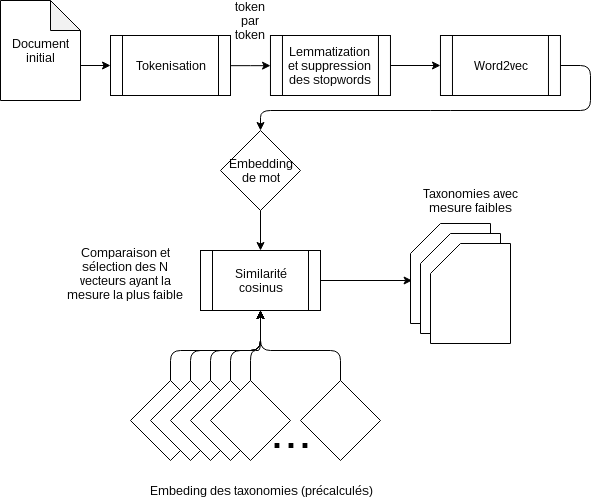
\includegraphics[width=0.8\textwidth]{taxoSchemaFoncInit.png}
	\caption[]{Schéma fonctionnel du module d'assignement taxonomique initial}
  \label{taxoInit}
\end{figure}


Nous avons rencontrés deux problème majeurs avec cette technique. D'abord, le temps d'execution de cette méthode pour un seul document sur le texte en entier dépassait largement les limites de l'acceptable. En effet, un document administratif est presque par nécessité très verbeux, et donc long. La majorité du texte ne nous est cependant pas utile pour notre but; il ne sert qu'à donner du contexte pour le lecteur et ne donne pas forcément d'information concernant le sujet du document en lui même. 

Deuxièmement, nous n'avons pas pu obtenir les résultats escomptés. Le principal obstacle venant du fait que les mots de la taxonomie peuvent être en fait des phrases, ou tout du moins de multiples mots dont les sens ne sont pas forcément corrélés. On trouve par exemple "amménagement foncier", mais aussi "fromage au lait cru" ou bien encore "médecine physique et de réadaptation". La technique que nous utilisions pour obtenir les \textit{embeddings}, word2vec, ne fonctionne pas sur des \textit{groupes de mots} ou \textit{n-grammes}, mais sur des mots seuls. doc2vec, qui lui peut fonctionner sur des n-grammes, voires des paragraphes ou documents entier a besoin d'être entrainé sur des documents qui lui apporteront le contexte nécessaire pour former des \textit{embeddings} correct. Cependant, la taxonomie ne donne aucun contexte. Il s'agit seulement d'une liste de mot et de phrase ordonnée seulement sous la forme d'un arbre. Il ne s'agit pas d'un document ordinaire, et nous pouvions pas utiliser les techniques courantes dans ce cas. 

Pour essayer de contrer ce problème, la décision initale fut de transformer chaque mot de la phrase en sa racine par le procédé de la lemmatization a l'aide de la librairie spacy\cite{spacy} et d'enlever les \textit{stopwords} de la phrase. Les \textit{stopwords} sont des mots apparant très fréquement dans les phrases, comme les déterminants. Ainsi la phrase "médecine physique et de réadaptation" se trouve transformée en "médecine physique réadaptation". On utilise ensuite un word2vec sur chaque mot pour obtenir plusieurs vecteurs. Pour obtenir un seul vecteur que nous comparerons avec les mots du documents, nous effectuons un simple moyennage. Cependant, cette solution n'as pas fonctionné et les taxonomies que nous trouvions a l'aide de ce système ne correspondait simplement pas au document. 

La solution finale adaptée fut celle de simplement extraire les titres d'arrétées administratifs, qui sont les documents a classer, et a les prétraiter par lemmatization et élimination des stopwords avant d'effectuer une simple recherche dans la taxonomie. Si un mot de la taxonomie se trouve dans le titre de l'article administratif, alors celui ci est ajouté au document. Cette solution est non seulement bien plus simple et permet de vérifier la qualité des résultats plus aisément qu'à l'aide d'un \textit{embedding}, et elle est de plus bien plus rapide, permettant l'analyse d'un document entier en quelques secondes a peine contre plusieurs minutes a l'aide d'un word2vec.


\begin{figure}[h!]
  \centering
  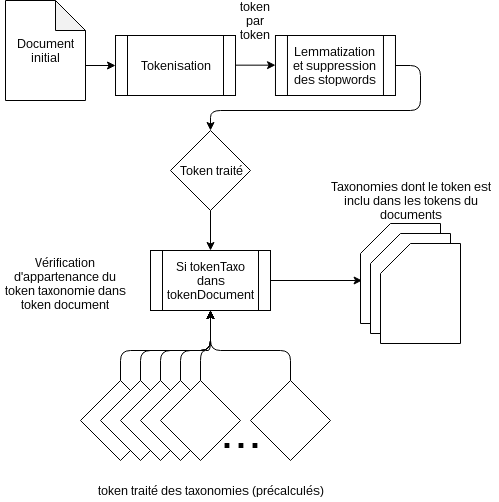
\includegraphics[width=0.8\textwidth]{diagFinalTaxo.png}
	\caption[]{}
  \label{}
\end{figure}

\subsection{Recherche de mots d'importance} %Baptiste
\subsection{Moteur de recherche} %Stab
